\documentclass[review]{elsarticle}

\usepackage{lineno,hyperref}
\usepackage{longtable}
\modulolinenumbers[5]

\journal{Journal of \LaTeX\ Templates}

%%%%%%%%%%%%%%%%%%%%%%%
%% Elsevier bibliography styles
%%%%%%%%%%%%%%%%%%%%%%%
%% To change the style, put a % in front of the second line of the current style and
%% remove the % from the second line of the style you would like to use.
%%%%%%%%%%%%%%%%%%%%%%%

%% Numbered
%\bibliographystyle{model1-num-names}

%% Numbered without titles
%\bibliographystyle{model1a-num-names}

%% Harvard
%\bibliographystyle{model2-names.bst}\biboptions{authoryear}

%% Vancouver numbered
%\usepackage{numcompress}\bibliographystyle{model3-num-names}

%% Vancouver name/year
%\usepackage{numcompress}\bibliographystyle{model4-names}\biboptions{authoryear}

%% APA style
%\bibliographystyle{model5-names}\biboptions{authoryear}

%% AMA style
%\usepackage{numcompress}\bibliographystyle{model6-num-names}

%% `Elsevier LaTeX' style
\bibliographystyle{elsarticle-num}
%%%%%%%%%%%%%%%%%%%%%%%

\begin{document}

\begin{frontmatter}

\title{Elsevier \LaTeX\ template\tnoteref{mytitlenote}}
\tnotetext[mytitlenote]{Fully documented templates are available in the elsarticle package on \href{http://www.ctan.org/tex-archive/macros/latex/contrib/elsarticle}{CTAN}.}

%% Group authors per affiliation:
\author{Elsevier\fnref{myfootnote}}
\address{Radarweg 29, Amsterdam}
\fntext[myfootnote]{Since 1880.}

%% or include affiliations in footnotes:
\author[mymainaddress,mysecondaryaddress]{Elsevier Inc}
\ead[url]{www.elsevier.com}

\author[mysecondaryaddress]{Global Customer Service\corref{mycorrespondingauthor}}
\cortext[mycorrespondingauthor]{Corresponding author}
\ead{support@elsevier.com}

\address[mymainaddress]{1600 John F Kennedy Boulevard, Philadelphia}
\address[mysecondaryaddress]{360 Park Avenue South, New York}

\begin{abstract}
This template helps you to create a properly formatted \LaTeX\ manuscript.
\end{abstract}

\begin{keyword}
\texttt{elsarticle.cls}\sep \LaTeX\sep Elsevier \sep template
\MSC[2010] 00-01\sep  99-00
\end{keyword}

\end{frontmatter}

\linenumbers

\section{Introduction}

Since the dawn of internet and world wide web, humanity has witnessed a degree of connection beyond reckoning. The proliferation of digital devices pervaded with various applications that account for almost all aspect of humanity, have created cyber communities that constantly mutate \cite{AtaeiACIS}; \cite{AtaeiBigDataEnvirons}. In a world where we have network infrastructures that can support up to 250Mbps of data transmission, and smart phones and IOT devices that can have processing power of up to 3 Ghz, data becomes ubiquitous, the quantum that lays the foundation of the nexus \cite{AtaeiApsec}. 

According to InternetLiveStates.com \cite{internet2019internet}, only in one second, there are 9,878 tweets sent, 1,138 instagram photos uploaded, 3,117,720 emails sent, 99,738 Google searches made, and 94,144 Youtube videos viewed. That is, if it has taken 5 second the read the preceding paragraph, during that time, 15,588,600 emails are sent. 

Driven by the ambition to harness the power of this deluge of data, the term 'Big Data' (BD) was coined \cite{lycett2013datafication}. BD initially emerged to address the challenges associated with various characteristics of data such as velocity, variety, volume and variability \cite{AtaeiBigDataEnvirons}. BD is the practice of extracting patterns, theories, and predictions from a large set of structured, semi-structured, and unstructured data for the purposes of business competitive advantage \cite{AtaeiHype}; \cite{Huberty}. BD is a game-changing innovation, heralding the dawn of a new data-oriented industry. 

Nonetheless, BD is not a magical wand that can enchant any business process. While a lot of opportunities exist in BD, subsuming an emergent and rather high-impacting technology like BD to current state of affairs in organizations, is a daunting task. According to recent survey from Databricks, only 13\% of the organizations excel at delivering on their data strategy \cite{DataBricksSurvey}. Another survey by NewVantage Partners indicated that only 24\% organization have successfully gone data-driven \cite{NewVantageSurvey}. This survey also states that only 30\% of organizations have a well established strategy for their big data endeavour. In addition, surveys from McKinsey \& Company (\cite{analytics2016age}) and Gartner (\cite{Nash}) further support these numbers, which illuminates on the scarcity of successful big data implementations in the industry.

Among the challenges of data adoption perhaps the most highlighted are 'data engineering complexities', 'big data architecture', 'rapid technology change', 'lack of sufficient skilled data engineers', and 'organization's cultural challenges of becoming data-driven' \cite{AtaeiBigDataEnvirons};\cite{Singh}. This focus of this study is on data engineering complexities and in specific big data architecture.

In the past, organization relied on a few technology giants to provide infrastructure and tools necessary for big data, while today there's a plethora of choice from hundreds of providers covering different aspect of data ecosystem from ingestion, to logging, to stream processing, and to visualization \cite{NewVantageSurvey}. Companies are tending more and more towards Cloud-native architectures for cost reduction, improved efficiency and new roles have been introduced such as chief analytics officer (CAOs) amd chief data officers (CDOs) to channel the organizational big data capabilities toward business value and competitive advantage \cite{rad2017evaluating}. 

So how can one embark on this rather sophisticated journey? what can be a good logical approach to absorb the ever-increasing complexity of big data systems? how can organizations build different stacks to handle data for various workloads such as machine learning (ML), business analytics, data engineering, and streaming? 

We suggest that majority of the challenge discussed starts with data architecture \cite{AtaeiACIS}; \cite{AtaeiApsec}. The data ingestion, processing and consumption of different data workloads vary, and sometimes they don't go well together. A company that enacted a data lake and a data warehouse and tries to account for both ecosystems, can be dealing with immense complexity, which in turns impact data teams, which in turn can hinder innovation, create barriers and result in monumental  lost.

Development and deployment of an efficacious big data system is only the beginning of a big data journey. As data sources increase, variety of data increases, number of data consumers increase, the data store gets confuscated, and this can introduce threats for scalability and maintainability of the system. This also implies that only a handful of hyper-specialized data engineers would understand the system internals, creating silos, and potential miscommunication. 

Majority of these systems are developed on-premise as ad-hoc complicated solutions that do not adhere to the practices of software engineering and software architecture \cite{Gorton}; \cite{Nadal}. As the ecosystem grows and new technologies and data processing techniques are introduced, the software architect will have a harder time to come up with a solution that address the problem requirements. 

This can potentially create grounds for an immature architecture that results in solutions that are hard to scale, hard to maintain, and raise high-entry blockades \cite{AtaeiApsec}. Since the approach of ad-hoc design to big data system development is not desirable and may leave many architects and data engineers in the dark, novel data architectures that are designed specifically for BD are required. To contribute to this goal, we explore the notion of reference architectures (RAs) and present a distributed domain-driven software RA for big data systems.


\section{Why reference architecture?}

To justify why we have chosen reference architectures as the suitable artefact, first we have to clarify two assumptions; 

\begin{enumerate}
    \item having a sound software architecture is essential to the successful development and maintenance of software systems
    \item there exist a sufficient body of knowledge in the field of software architecture to support the development of an effective RA 
\end{enumerate}

One of the focal tenets of software architecture is that every system is developed to satisfy a business objective, and that the architecture of the system is a bridge between abstract business goals to concrete final solutions \cite{SoftwareArchitectureKazman}. While the journey of big data can be quite challenging, the good news is that a software RA can be designed, analyzed and documented incorporating best practices, known techniques, and patterns that will support the achievement of the business goals. In this way, the complexity can be absorbed, and made tractable.  

Practitioners of complex systems, software engineers, and system designers have been frequently using reference architectures to have a collective understanding of system components, functionalities, data-flows and patterns which shape the overall qualities of system and help further adjust it to the business objectives \cite{Cloutier}; \cite{kohler2019towards}. There is a fair amount of literature on reference architectures, and whereas different authors definition may vary, they all share the same tenets. 

A reference architecture is amalgamation of architectural patterns, standards, software engineering techniques that bridge the problem domain to a class of solutions. This artefact can be partially or completely instantiated and prototyped in a particular business context together with other supporting artefact to enable its use. RAs are often created from previous RAs and architecture \cite{AtaeiACIS}.

The usage of RAs for the development of complex systems is not new. In software product line (SPL) development, RAs are generic artifacts that are configured and instantiated for a particular domain of systems \cite{Derras}. In software engineering, major IT giants like IBM has referred to RAs as the 'best of best practices' to address unique and complex system development challenges \cite{Cloutier}. 

Based on the premises discussed and taking all into consideration, RAs can facilitate the issues of big data architecture and data engineering because of the following reasons;

\begin{enumerate}
    \item RAs can promote adherence to best practice, standards, specifications and patterns
    \item RAs can endow the data architecture team with openness and increase operability, incorporating architectural patterns that ensue desirable predefined quality attributes
    \item RAs can be the best initial start to the big data journey, capturing design issues when they are still cheap
    \item RAs can bring different stakeholders on the same table and help achieve consensus around major technological constructs
    \item RAs can be effective in identifying and addressing cross-cutting concerns
    \item RAs can serve as the organizational memory around design decisions, enlightening next subsequent decisions 
    \item RAs can act as a summary and blueprint in the portfolio of software engineers and architect, resulting in better dissemination of knowledge
\end{enumerate}

\section{Research Methodology}

There are a few studies that have addressed the systematic development of reference architectures. Cloutier et al \cite{Cloutier} present a high-level model for RA development through collection of contemporary information and capturing the essence of architectural advancements. In another effort,PuLSE-DSSA is proposed by Bayer et al. \cite{bayer2004definition} in the context of product line development and domain engineering. PulSE-DSSA emphasizes on capturing the existing architectural knowledge. Stricker et al. \cite{stricker2010creating} propose a pattern-based approach for creating an RA. This study revolves around software engineering patterns motivated by the work of Gamma et al  \cite{gamma1995design}; proposing a structural approach that includes three layers of patterns with well-defined hierarchical relationships. Nakagawa, Martins, Felizardo, and Maldonado \cite{nakagawa2009towards} propose an approach to RA design outside of product line management context that is concentrated towards aspect-oriented systems. 

Galster and Avgeriou \cite{galster2011empirically} propose an empirically grounded reference architecture based on two main facets; Existing RAs in practice and available literature on RAs. Along the same vein, Nakagawa et al \cite{nakagawa2014consolidating} presented ProSA-RA which is a 4 phase methodology that unlike many other methodologies do provide a more comprehensive instructions on RA evaluation. In addition, this methodology benefits from an ecosystem of complementary constructs that aid in RA design and evaluation such as RAModel \cite{nakagawa2012ramodel} and a framework for evaluation of RAs (FERA) \cite{santos2013checklist}.In a recent study, Derras et al. \cite{derras2018reference} propose a schema of practical RA development in the context of software product line and domain engineering. This study is based on capturing knowledge from architectures in practice with attention to variability, configurability and product line development. The findings provide a four-phase process to develop quality driven reference architectures. This approach is influenced by ISO/IEC 26550 \cite{wg2015iso}.

By analysis and study of all these approaches for design and development of RAs, a common pattern has been witnessed. Whereas some of them are more recent and some belong to years ago, there are commonalities that has been observed. All these approaches are grounded on three main pillars, 1) Existing RAs 2) RAs in literature 3) Architectures in practice. Taking this into consideration and by analyzing the results of the systematic literature review conducted by Ataei et al \cite{AtaeiACIS} we found'Empirically-grounded reference architectures' proposed by Galster and Avgeriou \cite{galster2011empirically}, a suitable methodology, because firstly it's been adopted by many studies, and secondly it's comparatively in-line with the nature of our study. 

Nevertheless, we did not fully adopt this methodology and rather customized to the needs of this particular research. This is due to some inherent limitations that has been witnessed with the methodology. For instance we could not find a comprehensive guideline on how to identify data sources and how it could be categorized and synthesized into the creation of the RA in the third step of the methodology, therefore we employed the Nakagawa's information source investigation guidelines and the overall idea of the RAModel. Another limitation we've faced was with evaluation of the RA. As evaluation, second to a sound research methodology is one of the key elements of any good design science research, we had to look for a stronger and more systematic evaluation approach than what was discussed in 'empirically grounded RAs' methodology. For this purpose, and inspired by the works of Angelov et al \cite{angelov2008towards}; \cite{angelov2014extending}, we first created an prototype of the RA in practice, and then used 'The architecture tradeoff analysis method' (ATAM) \cite{kazman1998architecture} to evaluate the artefact.

This research methodology is constituent of 6 phases which are respectively; 1) Decision on the type of the RA 2) Design strategy 3) Empirical acquisition of data 4) Construction of the RA 5) Enable RA with variability 6) Evaluation of the RA. The phrase 'empirically grounded' refers to two major elements; firstly the reference architecture should be grounded in well-established and proven principles; secondly, the reference architecture should be evaluated for applicability and validity. These don't only belong to Galster and Avgeriou methodology, and other researchers such as Cloutier \cite{Cloutier} and Derras et al \cite{Derras} have promoted the same ideas. 

It is worth mentioning that this methodology is iterative, meaning that the results gained from the evaluation phase (6th phase) determines the subsequent iterations until the design reaches saturation.

\subsection{Step1: Decision on type of the RA}

Precursor to any effective RA development, is the decision on type of it. The type of the RA is significant, as it illuminates on information to be collected and the construction of the RA in later phases. The selection on the type of RA for the purposes of this study is based on two dimensions; the classification framework proposed by Angelov et al. \cite{angelov2009classification} and the usage context \cite{angelov2008contracting}. 

Based on the classification framework proposed by Angelov et al. \cite{angelov2009classification}, five types of RA are defined. This framework has been developed with the goal of supporting analysis of RAs with regards to context, goal, and the architecture specification/design relationships. It is based on 3 major dimensions namely context, goals, and design, each having their own corresponding sub-dimensions. These dimensions and sub-dimensions are derived by the means of interrogatives (the usage of interrogates is a well-established practice for problem analysis (the usage of interrogates is a well-established practice for problem analysis). 

The interrogatives ‘When’, ‘Where’, and ‘Who’ have been used to address the ‘context’, ‘Why’ has been used to address ‘goal’, and ‘How’ and ‘What’ have been used to address ‘design’ dimension. The outcome of the study categorizes RAs in two major groups; 1) standardization RAs and 2) Facilitation RAs. This framework has been chosen because it is completely in-line with the purposes of this study and aims to demarcate a clear domain for the RA to be developed. The comprehensive classification of the RAs with examples in practice illuminates on how different RAs are playing roles in the industry and how they are classified. This brings clarity on what should be developed and what boundaries should be drawn.  

By reading the results of the recent SLR conducted by Ataei et al on BD RAs \cite{AtaeiACIS}, we've added more examples of the RAs on top of what was provided by Angelov \cite{angelov2009classification}, and provided the following updated list of RA classifications with examples;

\begin{enumerate}

    \item Standardization RAs
    
    \begin{enumerate}
      \item Type 1: classical, standardization architectures designed to be implemented in multiple organizations. Examples are: 
      
      \begin{enumerate}
        \item WRM \cite{hollingsworth1995workflow}
        \item OSI RM \cite{zimmermann1980osi}
        \item OATH \cite{OATH}
        \item COBRA \cite{pope1998corba}
        \item Neomycelia \cite{AtaeiApsec}
        \item Kappa \cite{kreps2014questioning}
        \item Bolster \cite{Nadal}
      \end{enumerate}

      \item Type 2: classical, standardization architectures designed to be implemented in a single organization 
      \begin{enumerate}
          \item Fortis Bank Reference Software Architecture \cite{angelov}
      \end{enumerate}
    \end{enumerate}

    \item Facilitation  RAs
    \begin{enumerate}   
        \item Type 3: classical, facilitation reference architectures for multiple organizations designed by a software organization in cooperation with user organizations
        \begin{enumerate}
            \item Microsoft Application Architecture for .Net  \cite{microsoft2002application}
            \item IBM PanDOORA
            \item OATH \cite{OATH}
            \item COBRA \cite{pope1998corba}
        \end{enumerate}

        \item Type 4: classical, facilitation architectures designed to be implemented in a single organization
        \begin{enumerate}
            \item Achmea Software Reference Architecture   \cite{greefhorst2006achmea}
            \item ABN-AMRO Web Application Architecture \cite{greefhorst1999een}
        \end{enumerate}
        
        \item Type 5: preliminary, facilitation architectures designed to be implemented in multiple organizations
        \begin{enumerate}
            \item ERA   \cite{angelov2008contracting}
            \item AHA   \cite{wu2002reference}
            \item eSRA  \cite{norta2007exploring} 
        \end{enumerate}
    \end{enumerate}
  \end{enumerate}

The domain driven distributed BD RA chosen for the purposes of this study pursues two major goals; 1) enabling and support the development and data engineering of big data systems 2) concurrently ensuring that interoperability between different heterogeneous components of the big data system is established. Therefore, the outcome artefact will be a BD RA that is a classical standardization RA designed to be implemented in multiple organizations. 

\subsection{Step2: Selection of Design Strategy}

Angelov et al \cite{angelov2008towards} and Galster et al\cite{galster2011empirically} have both presented that RAs can have two major design strategies to them; 1) RAs that are designed from scratch (practice driven), 2) RAs that are based on other RAs (research driven). Designing RAs from scratch is rare, and usually takes place in an emergent domain that have not perceived a lot of attention. On the other hand, most RAs today are the amalgamation of a priori concrete architectures, models, patterns, best practices, and RAs, that together provide a compelling artefact for a class of problems.  

RAs developed from scratch tend to create more prescriptive theories, whereas RAs developed based on available body of knowledge tends to provide with more descriptive design theories. The RA designed for the purposes of this study is a research-based RA based on existing RAs, concrete architectures, and best practices. 

\subsection{Step 3: Empirical Acquisition of Data }

As aforementioned, due to the limitation witnessed by this research methodology, we have augmented this phase, and increase the systematicity and transparency of data collection and synthesis through various academic methods such as systematic literature review or SLR.

This phase is made up of three major undertakings; 1) identification of data sources; 2) capturing data sources; 3) synthesis of data sources.

\subsubsection{Identification of data sources}

To identify suitable data sources, we've employed the first step of ProSA-RA methodology, 'information source investigation'. This step is an endeavour to capture focal and ancillary knowledge and theories that revolve around the target domain, and lay the ground of RA development.

To unearth the architectural quanta, and to highlight gradations between various approaches to BD system development, we've selected most relevant sources as the followings; 

\begin{enumerate}
    \item{\bf{Practice-led conferences:}} given that majority of recent advancements for emerging technologies such as microservices architecture \cite{gan2019open};\cite{laigner2021data} \cite{dragoni2017microservices} and big data are coming from virtually hosted practice-led conferences, we've chosen some of the best conferences hold world-wide for the purposes of data collection. These conferences are 1) Qcon \cite{QCON} 2) State of Data Mesh by ThoughtWorks \cite{ThoughtWorks} 3) Worldwide Software Architecture Summit'21 \cite{Geekle} and 4) Kafka Summit Europe 2021 \cite{KafkaSummit}. Our objective was to capture the frontiers of software architecture and emerging approaches currently being practiced in IT giants such as Google, Facebook and Netflix. Among all the speech in these conferences, we looked for topics that entailed the keywords 'emergent software architecture trends', 'distributed software architecture', and 'big data software architecture'. We used the software Nvivo to code the transcripts from the conference videos. We used the aforementioned keywords as the codes and associated different texts, summative, essence-capturing sentences, evocative attributes to them. During this process, a new theme 'domain driven design' emerged. We added that into the list of codes as well.
    \item{\bf{Publications:}} in order to capture evidence from the body of knowledge, we conducted a systematic literature review (SLR), following the guidelines of PRISMA presented by Moher et all \cite{moher2015preferred}. The main objective of this SLR was to highlight common architectural constructs found among all the BD RAs. This SLR is build on top of our recent work \cite{AtaeiACIS} that covered all the RAs by 2020. 

    The initial SLR included IEEE Explore, ScienceDirect, SpringerLink, ACM library, MIS Quarterly, Elsevier, AISel as well as citation databases such as Scopus, Web of Science, Google Scholar, and Research Gate. The SLR search keywords used were ’Big Data Reference Architectures’, ’Reference Architectures in the domain of Big Data’, and ’Reference Architectures and Big Data’. We followed the exact methodology, but this time for the years 2021 and 2022. Our aim was to find out if there has been any new BD RA published during the years mentioned.

    By the result of this SLR, we've found 3 more BD RAs (\cite{AtaeiApsec}; \cite{castellanos2021smart}; \cite{sang2017simplifying}) and we've added two new standards (\cite{ISO20546}; \cite{ISO20547}) to further solidify our study. Converging these new SLR with the old, covering the years 2010-2022, we've pooled 89 literature in the primary phase, and another 10 by snowballing and citation searching. These 99 literature then went through our inclusion, exclusion and quality criteria. These criteria is as blow; 

    \begin{itemize}
        \item Inclusion criteria:
        \begin{enumerate}
            \item studies that entailed real-world scenarios or tend to solve a problem in practice
            \item qualitative or quantitative researches that intended to solve the industry gaps in big data system development and architecture
            \item studies that had strong evaluations, preferably those that created the artefact in an actual organizational setup
            \item explores the concept of RAs
            \item provides or builds up on thorough discussion on BD RAs, limitations, drivers, and the overall ecosystem
            \item is recent, within the years specified
            \item is a conference paper, journal paper, book, book chapter, white paper, dissertation or thesis
        \end{enumerate}
        \item Exclusion criteria:
        \begin{enumerate}
            \item the study is not well evaluated or practice driven
            \item is a duplicate
            \item the study is not in-line with research objectives
            \item not written in English
            \item provides a poor quality or misleading technical information
        \end{enumerate}
        \item EQuality assessment:
        \begin{enumerate}
            \item is the study rich in terms of relevance to practice?
            \item does the study create related design/design science or kernel theories?
            \item does the study entail sufficient data? 
            \item does the study discuss the recent trends in BD domain?
            \item is the study based on primary data and is internationally focused?
        \end{enumerate}
    \end{itemize}
\end{enumerate}

\subsubsection{Data Synthesis}

After pooling the studies, we removed 11 studies before screening because either they were duplicates or they were not in English. The remaining 78 studies went through screen, in which, 2 studies excluded based on the exclusion criteria. From there on, 76 studies have been assessed for eligibility based on the quality framework and the inclusion criteria. The result of this process handed over 67 studies from this branch. From the other branch, 10 records identified through citation searching. These reports have been assessed through the same quality framework, inclusion and exclusion criteria, which yielded 5 studies from this stream. Together 68 studies pooled for this SLR as depicted in figure \ref{fig:PRISMA}.

\begin{figure}[h!]
    \centering
    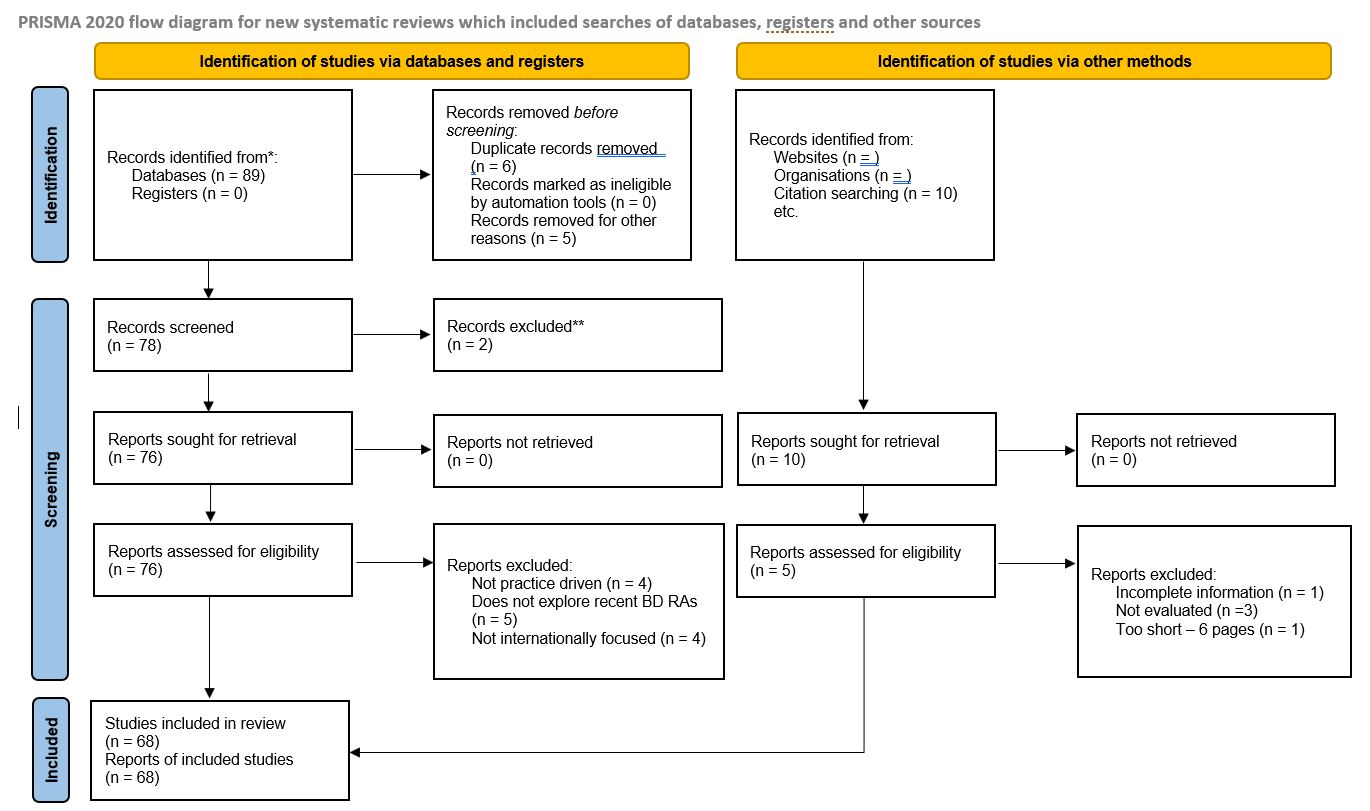
\includegraphics[width=10cm]{PRISMA.JPG}
    \caption{PRISMA flowchart}
    \label{fig:PRISMA}
\end{figure}


These 68 studies are comprising of journal papers, conference papers, book chapters, tech reports, tech surveys white papers, standards, master thesis, and PhD dissertations. Out of the pool of these studies, 39.4\% are from IEEE Explore, 4.4\% are from ScienceDirect, 23.5\% are from Springerlink, 13.2\% are from ACM, and 29.4\% are from other sources such as citation search, Google Scholar and Research Gate. 30 journal articles, 14 conference papers, 6 whitepapers, 2 ISO standards, 14 book chapters, and 2 postgraduate studies have been selected. 26\% of these studies are from the year 2010-2013, 33\% are from the years 2013-2015, and 51\% are from the years 2016-2022. These stats are portrayed in figure \ref{fig:SLRStats}. 

\begin{figure}[h!]
    \centering
    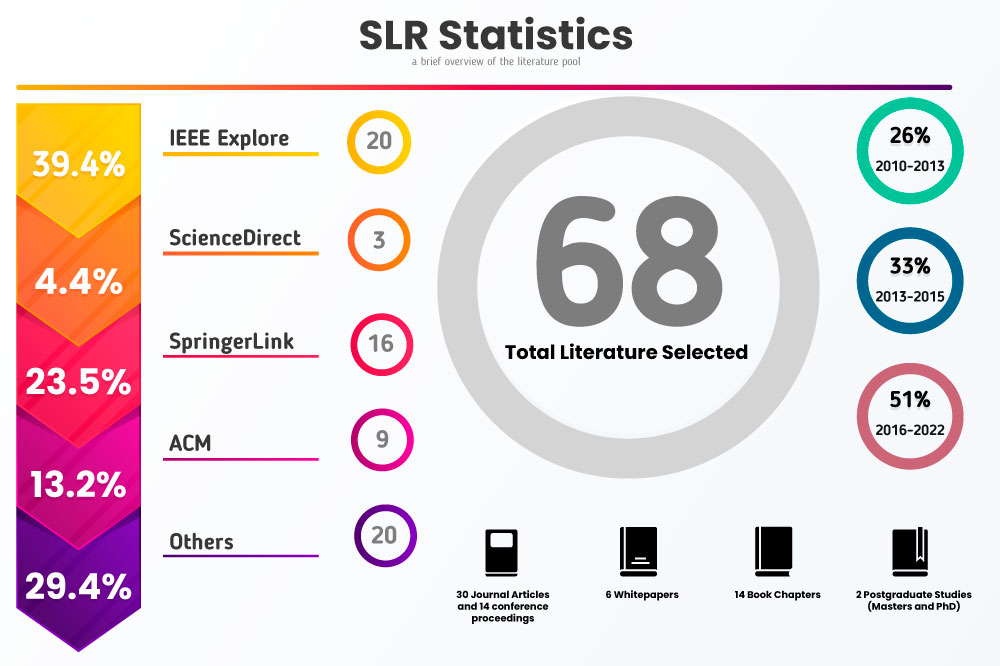
\includegraphics[width=11cm]{databases-statitistic.jpg}
    \caption{SLR statistics}
    \label{fig:SLRStats}
\end{figure}


By this stage, the research objective is set, studies are pooled, assessed and refined, thus the research embarked on the actual synthesis of data. To increase transparency, RAs and standards found as the result of this SRL is presented in table \ref{table:SLR}. For this purposes, the software Nvivo \cite{nvivo} has been used to code, label, and classify studies. Initially, all the keywords aforementioned has been created as nodes in the software, which are then associated to relevant sentences in studies. After coding all the studies, the findings have been synthesized to create theories, which in turn emerged themes and patterns. The findings gained from this SLR grounded the foundation for various aspect of the SLR development. 



    \begin{longtable}{|p{5cm} | p{1cm}  | p{1cm} | p{3.4cm}|} 
     \hline
     Study  & Author & Year & Type \\ [0.5ex] 
     \hline
     Towards a big Data reference architecture  & \cite{Maier}& 2013 & Master's Dissertation \\ 
     \hline
     A reference architecture for Big Data solutions introducing a model to perform predictive analytics using Big Data technology  & \cite{geerdink2013reference}  & 2013 & Conference Paper \\
     \hline
     IBM - Reference architecture for high performance analytics in healthcare and life science  & \cite{quintero2019ibm} & 2013 & Book \\ [1ex] 
     \hline
     Big data ecosystem reference architecture  & 
     \cite{levin2013big} & 2013 & White Paper \\ [1ex] 
     \hline
     A proposal for a reference architecture for long-term archiving, preservation, and retrieval of Big Data  & \cite{viana2014proposal}  & 2014 & Conference Paper \\ 
     \hline
     Questioning the Lambda architecture; Kappa Architecture  & \cite{kreps2014questioning}  & 2014 & Blog \\
     \hline
     Defining architecture components of the Big Data Ecosystem  & \cite{demchenko2014defining} & 2014 & Conference Paper   \\ [1ex] 
     \hline
     Oracle - Information Management and Big Data: A Reference Architecture   & 
     \cite{cackett2013information} & 2014 & White Paper \\ [1ex] 
     \hline
     Big Data driven e-commerce architecture   & \cite{ghandour2015big} & 2015 & Journal Article \\ [1ex] 
     \hline
     The solid architecture for real-time management of big semantic data & \cite{martinez2015solid} & 2015 &  Journal Article \\ [1ex] 
     \hline
     Reference architecture and classification of technologies, products and services for big data systems  & \cite{paakkonen2015reference}  & 2015 & Journal Article \\ [1ex] 
     \hline
     A Reference Architecture for Big Data Systems  & \cite{sang2016reference}  & 2016 & Conference Paper  \\  
     \hline
     A reference architecture for Big Data systems in the national security domain  & \cite{klein2016reference}  & 2016 & Conference Paper \\ [1ex] 
     \hline
     A Reference Architecture for Supporting Secure Big Data Analytics over Cloud-Enabled Relational Databases  & \cite{cuzzocrea2016reference}  & 2016 & Conference Paper \\ [1ex] 
     \hline
     SAP - NEC Reference Architecture for SAP HANA \& Hadoop   & 
     \cite{SAPRA} & 2016 & White Paper \\ [1ex] 
     \hline
     Managing Cloud-Based Big Data Platforms: A Reference Architecture and Cost Perspective  & \cite{heilig2017managing} & 2017 & Journal Article \\ [1ex] 
     \hline
     Scalable data store and analytic platform for real-time monitoring of data-intensive scientific infrastructure   & \cite{heilig2017managing} & 2017 & PhD Dissertation \\ [1ex] 
     \hline
     A software reference architecture for semantic-aware Big Data systems; Bolster Architecture   & \cite{nadal2017software} & 2017 & Journal Article \\ [1ex] 
     \hline
     Simplifying big data analytics systems with a reference architecture
     & 
     \cite{sang2017simplifying} & 2017 & Conference Paper \\ [1ex] 
     \hline
     ISO/IEC/IEEE 42010:2011 & \cite{ISO42010} & 2017 & Standard \\ [1ex] 
     \hline
     NIST Big Data Interoperability Framework: Volume 6, Big Data Reference Architecture
     & \cite{Chang} & 2018 & White Paper \\ [1ex] 
     \hline
     Towards a secure, distributed, and reliable cloud-based reference architecture for Big Data in smart   & \cite{kohler2019towards} & 2019 & Book Chapter \\ [1ex] 
     \hline
     Reference Architectures and Standards for the Internet of Things and Big Data in Smart Manufacturing   & \cite{unal2019reference} & 2019 & Conference Paper \\ [1ex] 
     \hline
     Lambda architecture & \cite{kiran2015lambda} & 2019 & Conference Paper \\ [1ex] 
     \hline
     ISO/IEC 20546:2019 & \cite{ISO20546} & 2019 & Standard \\ [1ex] 
     \hline
     ISO/IEC TR 20547-1:2020 & \cite{ISO20547} & 2020 & Standard \\ [1ex] 
     \hline
     NeoMycelia: A software reference architecturefor big data systems
     & 
     \cite{AtaeiApsec} & 2021 & Conference Paper \\ [1ex] 
     \hline
     Smart transportation: A reference architecture for big data analytics
     & 
     \cite{castellanos2021smart} & 2021 & Journal Article \\ [1ex] 
     \hline
     \caption{RAs and Standards found by the result of the SLR}
     \label{table:SLR}
    \end{longtable}
\subsection{Construction of the RA}

Based on the themes, theories, and patterns realized in the previous steps, the process of RA construction took place. Integral to this step was the identification of elements that the RA should contain, how these elements should be synthesized, and how the RA can be portrayed and communicated. To describe our RA, we followed ISO/IEC/IEEE 42010 standard \cite{ISO42010}. This standard pivots on concrete architectures, so we did not 100\% conform to it, but rather the good and relevant parts of it has been taken. For instance, architecture viewpoints, statement of corresponding rules, and expression of the architecture through architecture description languages (ADLs) have had direct aspects on the construction of this RA.

A key challenge in the development of this RA was to strike a balance between the specificity of the micro patterns and approaches to system development and general architectural concepts that reflect a view of a the system as an array of interrelated entities. Angelove et al \cite{angelov2012framework} approached this problem by the means of interrogative through a defined framework that aims to guide the creation of RAs.
Cloutier et al \cite{Cloutier} suggest that a RA should entail technical, business and customer context views, whereas Vogel et al \cite{vogel2009software} provided classifies RA views based on the usage context, as industry specific, platform specific, industry crosscutting and product line RAs. 

Stricker et al \cite{Stricker} expressed their pattern-based RA by adhering several distinct views into one. Chang et al \cite{Chang} presented NIST BD RA as system constituent of logical components connected though interoperability interfaces in several fabrics. On the other hand, ISO/IEC/IEEE 42010 refrains from using phrases such as “technical architecture”, “physical architecture”, or “business architecture”. 

Taking the best evidence from the available body of knowledge, We decided to adhere several views into one and it express the RA through a multi-layer modeling language called Archimate. Archimate is mature modeling language developed by the Open Group that provides with a uniform representation of high-level architectural diagram aimed at portraying and delineating Enterprise architecture \cite{lankhorst2013language}. Archimate being listed as a standard architecture description language in ISO/IEC/IEEE 42010, is designed based on a set of related concepts that are specialized towards the system at different architectural layers. This means that the architect is enhanced with an integrated architectural approach that visualizes and describes different architecture domains and their underlying relations \cite{lankhorst2010anatomy}; \cite{engelsman2011extending}. 

Archimate utilizes service-orientation to distinguish and relate the application, business and technology layer and use realization relationships to create relationship between concrete elements and more abstract elements across three layers. In addition, Archimate can be customized to account for varying needs of the architect.

\subsection{Enabling RA with variability}

Enabling RA with variability is an important process that helps with the instantiation of it. 
This allows RA to remain useful as a priori artefact when it comes to country-specific regulations, and organizational compliance that constrain the architect design decisions \cite{rurua2019representing}.

Variability management has been studied in the domain of Business Process Management (BPM) \cite{la2009questionnaire}; ;\cite{rosemann2007configurable}; \cite{hallerbach2010capturing} and Software Product Line Engineering (SPLE) \cite{pohl2005software}\cite{chen2011systematic}; \cite{schmid2004customizable}; \cite{svahnberg2005taxonomy}; \cite{sinnema2006covamof}. In BPM, variability management revolves around efficient handling of of different variants in business processes, whereas in SPLE, variability management is about modifying and extending the software artefact to account of the requirements of a specific context.

Clear identification of variability and explicit communication of it improves communication between stakeholders, allows for traceability between variation causes and effects and facilitates the decision making \cite{czarnecki2012cool}. 

Variation points are decided based on the data collected in previous steps. Galster et al \cite{galster2011empirically} sugguest that there are three approaches to enabling variability;

\begin{enumerate}
    \item Annotation of the RA
    \item Variability views 
    \item Variability models
\end{enumerate}

We could not find an in-detail explanation of how one should choose the appropriate variability enabling approach. Therefore, inspired by the works of Rurua et al \cite{rurua2019representing}, we decided to extend the RA with variability, by the means of Archimate annotations. We have achieved this in two steps; first we developed a custom layer that represents focal variability concepts, and then we extended the RA through annotation. The aim of this process is not find all variability points that may emerge in the usage context, but to provide with high-level system related architectural variabilities that an architect may consider for improvement of design and adoption of the RA.

The variability model is depicted in Fig \ref{variability} by the means of Archimate's motivation layer. This modeling is driven by the works of Pohl et al \cite{pohl2005software} and in specific their graphical notation of variability information, and Rurua et al \cite{rurua2019representing} and in specific, their variability management concepts model.

\begin{figure}[h!]
    \centering
    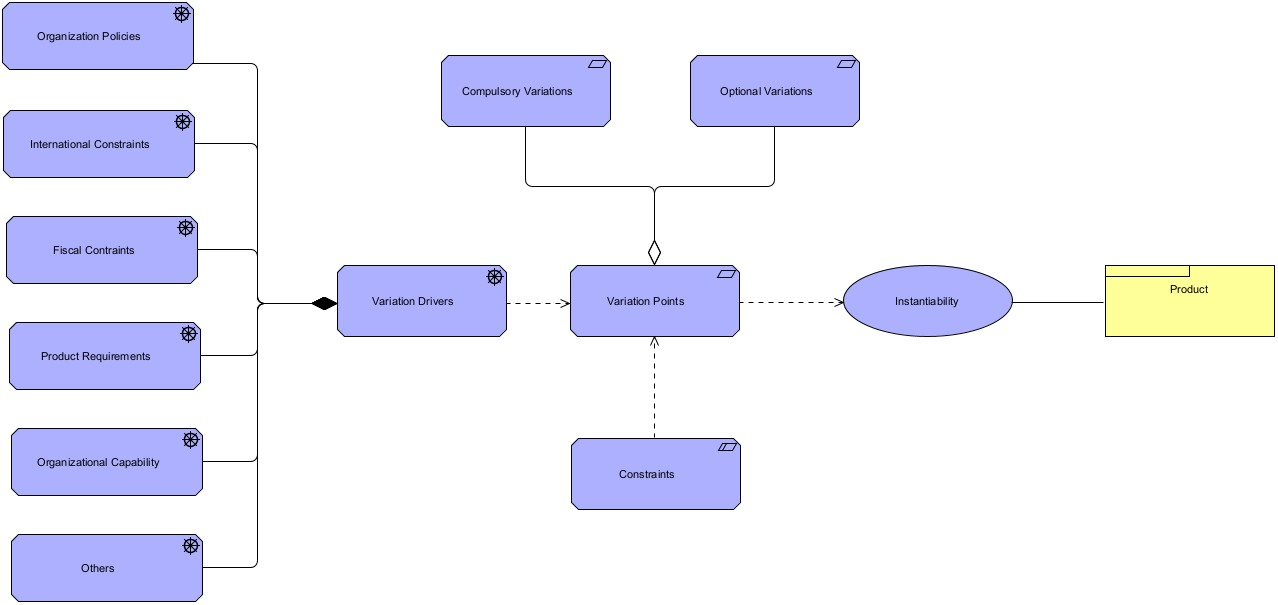
\includegraphics[width=11cm]{variability-model.JPG}
    \caption{Variability management concepts model}
    \label{variability}
\end{figure}

\subsection{Evaluation of the RA}

Evaluation of the RA is to ensure that it has achieved the goals stated prior to development, to test is effectiveness and usability, and to make sure that it addresses the identified problems. Two fundamental pillars of the evaluation is the correctness and the utility of the RA and how efficient it can be adapted and instantiated \cite{galster2011empirically}. The quality of RA can be assessed by how it can be transformed into an effective organization-specific concrete architecture. The fact that this RA is built upon former RAs helps making the evaluation steps easier as the research can get inspiration from other studies and their approach to evaluation \cite{sharpe2019industrial}. 

Nevertheless, evaluation of the RAs is a well-known challenge among researchers \cite{angelov2008contracting}; \cite{Avgeriou}; \cite{Cioroaica}; \cite{Maier}. RAs and concrete architectures have distinct qualities. They vary in at least 3 major ways; 

\begin{enumerate}
    \item RAs are of higher level of abstraction 
    \item in RAs stakeholders are not clearly grouped 
    \item RAs tend to be focused more on architectural qualities
\end{enumerate}

While there are many well-established methods for assessing concrete architectures such as Scenario-based Architecture Analysis Method \cite{kazman1994saam}, Architecture Level Modifiability Analysis \cite{Bengtsson}, Performance Assessment of Software Architecture \cite{Williams}, Architecture Trade-off Analysis Method \cite{KazmanATAM}, none of these methods can be directly applied to evaluate RAs. To support this statement, three major issues have been identified. These issues are as follows;

\begin{enumerate}
    \item One of the main problems for applying existing evaluation methods to RA is the lack of clearly defined group of stakeholders \cite{angelov2008towards}, while ATAM and other methods are highly dependent on participation of stakeholders for evaluation. Due to the level of abstractness of the RA, reaching various group of stakeholders and persuade them to anticipate in the study, is problematic and does not fit to the timeline of this study. Even more notably, it is unlikely that all stakeholders will unite around a common reference architecture as different members may or may not agree with the overall idea of the RAs, may come from different backgrounds, and may lack architectural visions 
    \item Evaluation frameworks and methods for concrete architectures make use of scenarios. Howbeit due to RAs level of abstraction, creation of usable scenario is difficult. Either a large set of scenarios should be developed covering all the aspects of the RA with regards to specific domain, or a more general scenarios should be developed to cover all the aspects. In the first approach, a large number of scenarios, makes data analysis troublesome and a tedious process. Moreover, the order of prioritization of these scenarios and defining them, and validating them is a problematic task. In the second approach, due to the generality of the scenario, evaluation of effectiveness and usability of the RA becomes difficult and may become incomplete \cite{Avgeriou}. These challenges have been observed even in the evaluation of highly complex concrete architectures in information systems domain \cite{bengtsson1998scenario}. 
\end{enumerate}

Based on the problems discussed above, available methods of architecture analysis are not sufficient in evaluating the RA. This has been addressed by various researchers in the industry. 

In one study, Angelov et al \cite{angelov2008towards}, modified ATAM and extended it to resonate well with RAs. This process took place by invitation of representatives from leading industries for the evaluation process, and the selection of various contexts and defined scenarios for these contexts. Furthermore, ATAM has been extended to evaluate completeness, buildability and applicability. Howbeit the selection of the right candidate and involving them in the process is a time-consuming and daunting task and may yield incomplete information. In addition, candidates maybe lacking architectural visions, increasing the threat to validity. 

In addition to extending ATAM for RAs, Graaf et al \cite{graaf2005evaluating} presented an evaluation approach in which SAAM is extended to help reduce the organizational impact of it. In Another study by Maier et al, Maier et al. (2013) as a postgraduate thesis in Eindhoven University of Technology, the evaluation of the RA has been conducted by mapping it against existing concrete architectures described in industrial whitepapers and reports. Along the lines, Galstar et al \cite{galster2011empirically} suggested reference implementations, prototyping and incremental approach for the validation of the RA. 

Rohling et al \cite{rohling2019reference} have evaluated their RA by mapping it against the requirements set for the study. This was facilitated by the RA research methodology created by Nakagawa et al \cite{Nakagawa} and the complementary RAModel \cite{nakagawa2012ramodel}.Inspired by all the studies listed, for the purposes of this study, we will first create a prototype of the RA in an actual organizational setup and then we will use ATAM to evaluate the concrete architecture. 

\section{Cybermycelium: A Domain Driven Distributed Reference Architecture for Big Data Systems}

If our aspiration to enhance every business aspect with data needs to com to fruition, we need a different approach to data architecture. Traditional data warehouse approaches to business intelligence, while have addressed the volume and computing aspect of data, they have failed to address other characteristics of it; heterogeneity and proliferation of data sources (variety), the speed at which data arrives and needs to be processed (velocity), the rate at which data mutates (variability), and the truth or quality of the data (veracity).

\subsection{State of the art}

The available body of knowledge and practice highlights 3 generations of big data architectures; 

\begin{enumerate}
    \item \textbf{Enterprise Data Warehouse:} this is perhaps one of the oldest approaches to business intelligence and data crunching and hast existed even before the term big data was coined \cite{leonard2011design}. Usually developed as proprietary software, this data architectures pivot on enterprise data warehouse, ETL jobs, and a data visualization software such as Microsoft Power BI. As the data sources and consumers grow, this architecture suffers from hard to main ETL jobs, and visualizations that can be created and understood by a certain group of stakeholders, hindering data's potential positive impact on business. 
    \item \textbf{Data Lake}: to address the challenges occurred in the first generation of data architectures, a new big data ecosystem emerged. This new ecosystem revolved around a data lake, in way that there isn't as much transformations on the data, but rather everything is dumped into the data lake and retrieved when necessary. Although data lake architecture have reached a higher level of success in comparison to the first generation of the data architectures, they are still far from optimal. As data consumer and data providers grow, data engineers will be immensely challenged to avoid creating a data swamp \cite{brackenbury2018draining}, and because there is usually no concept of data owner, the whole stack is usually operated by a group of hyper-specialized data engineers, creating silos, and barriers for gradual adoption. This also means various teams will often go into data engineers backlog and will not be in control of how and when they can consume the data they desire.
    \item \textbf{Cloud Based Solutions:} Given the cost and complexity of running a data lake on-premise alongside the whole data engineering pipeline, and the substantial talent gap currently faced in the market \cite{AtaeiHype}, the third generation of big data architectures tend to revolve around as-a-service or on-demand cloud-based solutions. This generation of architecture tends to be leaning towards stream-processing with architectures such as Kappa or Lambda \cite{lin2017lambda}, or frameworks that unify batch and stream processing such as Apache Beam \cite{ApachBeam} or Databricks \cite{DataBricks}. This is usually accompanied by cloud storage such as Amazon S3, and streaming technologies such as Amazon Kinesis. Whereas this generation tends to solve various issues regarding the complexity and cost of data handling and digestion, it still suffers from the same fundamental architectural challenges.
\end{enumerate}

To discuss the integral facets that embroil these architectures, one must look at the characteristics of these architectures and the ways in which they achieve their ends, with quality attributes surrounding it. Except for one case \cite{AtaeiApsec}, all the architectures and RAs found as the result of this study, were designed underlying monolithic data pipeline architecture with four major components being data consumer, data processing, data infrastructure and data providers. 

The process of turning data into actionable insights in these architectures usually follow a similar lifecycle;

\begin{enumerate}
    \item \textbf{Data Ingestion:} system beings to ingest data from all corners of the enterprise, including both transactional, operational and external data. For instance, in a practice management software for veterinaries, data platform can ingest and persist transactional data such as 'user interaction with therapeutics', 'number of animals diagnosed', or 'number of invoices created' and 'medicines dispensed'.
    \item \textbf{Data Transformation:} data captured from the previous step is then cleansed for duplication, quality, and potentially scrubbed for privacy policies. This data then goes through a multifaceted enrichment process to facilitate data analysis. For instance, a journey of the veterinary nurse can be captured at every stage, enriched with demographics and animal breed for regression analysis and aggregate views.
    \item \textbf{Data Serving:} at this stage, data is ready to be served to diverse array of needs ranging from machine learning to marketing analytics, to business intelligence to product analysis and customer journey optimization. In the 'veterinary practice management software' the data platform can provide real-time data through event backbone system such as Kafka  about customers who have applied and have been dispensed Restricted Veterinary Medicine (RVM) to make sure that these transactions comply with the conditions of the registration of these products.
\end{enumerate}

The lifecycle depicted is indeed a high-level abstract view of prevalent big data systems. Howbeit, it highlights an important matter; these systems are all operating underlying monolithic data pipeline architecture that tends to account for all sorts of data. This means, data that logically belong to different domains are now all lumped together and crunched in one architectural constructs, making maintainability and scalability a daunting task \cite{monolithToMesh}. 

While architectures in software engineering have gone through series of evolution in the industry, adopting a more decentralized and distributed approaches such as microservice architecture, event driven architectures, reactive systems, and domain driven design \cite{alshuqayran2016systematic}, the data engineering, and in specific big data ecosystems do not seem to be adopting many of these patterns. Evidence collected from this study have proven that attention to decentralized big data systems, metadata, and privacy is deficient. Therefore, the whole idea of 'monolithic data pipeline architecture with no clearly defined domains and ownership' brings significant challenges to design, implementation, maintenance and scaling of big data systems. 

Suppose company A would want to adopt a big data initiative to embark on this complex endeavour, what would be the first step ? does the company have to worry about high-throughput stream processing ? does it have to worry about regional privacy regulations? does it have to worry about cost-efficient batch processing? perhaps yes to all of these questions, but what's even more integral to the success of the whole endeavour is the underlying architecture that governs the entire system, its components, their relations to each other, data flow and principles and standards that govern the quality attributes and evolution of the system.

This architecture and design process if done underlying current prevalent approaches, can bring about colossal lost, and leave many managers disappointed. In fact, we don't claim that all these architectures will fail, perhaps some have proven to be successful in a specific context. There are two threats to maintainability and scalability of these systems; 

\begin{enumerate}
    \item \textbf{Data source proliferation:} as the big data system grows and more data sources are added, the ability to ingest, process, and harmonize all these data in one place diminishes. This in turn, reduces maintainability, makes company reliant on lead data engineers who built the infrastructure, and makes scaling these systems very difficult. The proliferation of data sources if not managed carefully, can result in data swamps as well, which makes understanding data domains, and providing data as a service a complicated task. 
    \item \textbf{Data consumer proliferation:} organizations that utilize rapid experimentation approaches such Hypothesis-Driven Development and Continuos Delivery \cite{hypothesisDev} constantly introduce new use cases for data to be consumed in different domains. This means that variability of the data rises, and the sum of aggregations, projections, and slices increases, which in turn adds more work to the backlog of the data engineering team, slowing down the process of serving the data to consumers. Inability to account for the data consumer demands can be a point of friction in organizations \cite{monolithToMesh}.  
\end{enumerate}

To address these challenges, the lead architect or the architecture governance group will then have to choose the right architectural quanta to segregate the monolith. According to Ford et al \cite{ford2017building}, an architectural quantum is a component of a system with high functional cohesion that is independently deployable, this is also referred to as a service \cite{newman2021building}. The main motivation for segregating the monolith into its architectural quantum, is to parallelize work in various business domain, to reach a better velocity, reduce cost, promote ownership, increase performance and reach higher operational scalability.

Currently, these architectures are usually segregated into pipelines that each process data differently. While each pipeline has its own responsibility to handle various aspect of the big data system, there is still a high coupling between the pipelines, as 'data cleansing' phase cannot start after 'data ingestion'. This coupling is even more highlighted when the company is at the stage of rapid experimentation with data sources and would like to explore new domains of insight generation, and this in turn means that delivering new features and values is orthogonal to the axis of change. 

Using the same practice management software example, given that a new class of animals (equine animals as opposed to small animals) should be incorporated for data analysis; the data engineering team should then modify and extend the whole pipeline of ingest, process and serve to account for the particularity of the data captured regarding this new class of animals. New ingestion services required, the schema might change, the veracity checking mechanisms might differ, cleansing varies and more. This implies an end-to-end dependency which affects external teams, slows down processes and make maintenance gradually harder. This implies that using pipeline as an architectural quantum in such a coupled way is perhaps not the most efficient architecture to big data systems. 

Another major issue with the current architectural approaches is that data engineering is usually confined into a team of hyper-specialized individuals who are siloed from the operational units of the organization. These teams, being fully responsible for creating the infrastructure for data processing, are often absent of business knowledge and the domain, which limits their productivity. These individual usually have a limited understanding of the data sources, data provenance, data consumers, the changing nature of the business domains, the overall product vision, and the application side of things, yet they are responsible to provide data for a large array of analytical and operational needs in a timely manner. For instance, given a context in which a product owner and application developer can cooperate, the synergy between the data engineer, application developer, and product owner can bring about more mature decisions that can align the requirements across various technical and logical domains and allow for various stakeholders to contend and communicate their concerns.

Whereas there could be other factors to be discussed deeply in this paper regarding current big data architectures, our aim is not to explore any further and emphasize more on the solution artefact we've designed to address some of these challenges. 

\section{A paradigm shift: distributed domain driven architecture}

Based on the premises discussed priori to this section, one can infer that the idea of monolithic and centralized data pipelines that are highly couped and operated by silos of hyper-specialized big data engineers has limitations and can bring organizations into a bottleneck . 

We therefore, explore a domain driven distributed and decentralized architecture for big data systems and posit that this architecture can address some of the challenges discussed. This idea is inspired by the advancements in software engineering architecture, and in specific event-driven microservice architecture \cite{EventDrivenMicroServices}, domain driven design \cite{evans2004domain}, and reactive systems \cite{aceto2007reactive}.

Data usually comes into two different flavours; 1) operational data which serves the need of an application, facilitates logic, and can include transactional data and 2) analytical data which usually has the temporality to it, and is aggregated to provide with insights. 

These two different flavours, despite being related, have different characteristics and trying to lump them together may result in a morass. To this end, Cybermycelium realizes the varying nature between these two planes and respects the difference. Cybermycelium aims to transfigure current architectural approaches by proposing an inversion of control, and a topology based on product domains and not the technology \cite{dataMeshArticle}. Our proposition is that handling two different archetypes of data, should not necessarily result in siloed teams, heavy backlogs, and a coupled implementation. 

To further elucidate on this matter, we take the example of the microservice architecture. As the industry sailed away from the monolithic n-tier architectures into Service Oriented Architectures (SOA), organizations faced a lot of challenges. One prevalent issue was around the maintenances of Enterprise Service Bus (ESB) or SOA bus, which is the locus of aggregation. While the aggregation layer could be written very thin, the reality is that the transformation of XML and logical operations started to bloat the SOA bus. This added a new level of coupling between internal and external elements of the system as a whole \cite{di2017architecting}; \cite{zimmermann2017microservices}; \cite{waseem2020systematic}. 

Microservices architecture, being the evolution of SOA, move away from smart pipelines into dumb pipelines and smart services removing the need for the locus of aggregation and control. Moreover, there was no business logic written in the pipelines, and each service was segregated usually with the help of domain driven design. 

Whereas microservices architecture still have its challenges, the gradations of software architectures in software engineering industry can be analogous to the data engineering domain. One can perceive the pipeline architecture and its coupling nature similar to SOA and the business logic written to connect the services in the SOA bus. 

Based on these premises we posit 4 underpinning principles for Cybermycelium; 

\begin{enumerate}
    \item Distributed Domain driven services with bounded context
    \item Data as a service
    \item Data infrastructure automation
    \item Governance through a federation service 

\end{enumerate}

\subsection{Distributed Domain driven services with bounded context}

Integral to Cybermycelium, is the distribution and decentralization of services into domains that have clear bounded context. Perhaps one the most challenging things one might face when it comes to architecting a distributed system is; based on what architectural quanta should we break down the system. This issue has been repeatedly discussed for example among adopters of microservices architecture . Cybermycelium, inspired by the concept of domain-drive design, tends to sit data close to the product domain that relates to it. This implies that data inheres in the product domain and as a facet of it \cite{laigner2021data}.

This is mainly driven by the fact that most organizations today are decomposed based on their products. These products are the capability of the business that are segregated into various domains. Domain's bounded context is operated by various teams with different visions and concerns, incorporating data into a bounded context can result in a synergy that can improve the management of evolution and continuos change. This can be micro, such as application developers communicating with data engineers about collecting user data in a nested data structures or in flat ones, or macro, such as application developers thinking about redesigning their graphql schema in an intermediary layer that may affect the data engineers ingestion services. 

\subsection{Data as a service:}

Data can be conceived as the fourth dimension of a product next to UI/UX, business and application (\ref{data-facets}). Each domain provides its data as a service. This data is consisting of both operational and analytical data. This also implies that any friction and coupling between data is removed. For instance, the 'invoice' domain will provide the transactional data about number of invoices and total of discounts with analytical data such as which practices have created what number of invoices in what period of time.

\begin{figure}[h!]
    \centering
    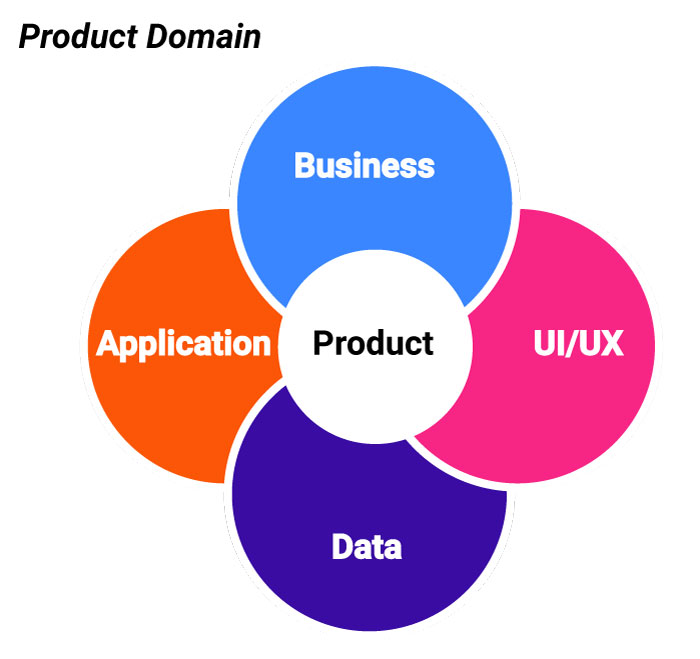
\includegraphics[width=10cm]{Media/product-facets.jpg}
    \label{data-facets}
    \caption{Product Facets}
\end{figure}

However this data-as-a-service model should be carefully implemented to account for explorability, discoverability, security, and quality. The data provided as a service should have the identical qualities to customer-facing products. This also implies, that a product owner should now treat data facet as an aspect of the product and employ objective measures that assure the desired quality. These measure can be net promoter scores from data consumers, data provenance, decreased lead time. Product owners, in addition to the application and design aspect of the product, must now incorporate this new facet, and try to understand the needs of the data consumers, how they consume the data, and what are the common tools and technologies they utilized to consume the data. This knowledge can help shaping better interfaces for the product.

Product domains may also need to ingest data from upstream domains, and this requires the definition of clear interfaces. Furthermore, each domain should also account for metadata. Metadata in derived from the nature of the product and its data lifecycle. Data can be ingested and served in various forms such as tables, graphs, JSON, events, and many more; but in order for the data to be useful for analytical purposes, there is a need to associate data with its corresponding metadata that encompasses semantics, and history. 

\subsection{Data infrastructure automation}

As the number of product domain increases, the effort required to build, deploy, execute, and monitor services increases. This includes the data pipelines required for that product domain to carry out its functions. The platform skills required for these kinds of work is usually found in Devops engineers and site reliability engineers. Application developers and data engineers are usually not adept at carrying out such workloads in an efficient manner. For this reason, there is a need for highly abstract reusable infrastructural components that can be easily utilized. This implies that teams should be equipped with required infrastructure as a service, that can be easily employed to account for big data needs.

One way to provision such infrastructure as a service, is to utilize infrastructure as a code software tools like Terraform \cite{Terraform}. Besides, data infrastructure may be extended based on currently running infrastructure for application payloads. However, this might be challenging, as the big data ecosystem is growing rapidly, and while a software application might be running in an EC2 worker node in an EKS cluster on Amazon, the big data system maybe running Databricks, a CDP solution like Segment \cite{Segment}, HDFS \cite{HDFS}, or Amazon Kinesis.This brings the challenge of composing data and application infrastructure together to provide with coherent, cost efficient interoperable infrastructure.  

Nevertheless, this should not be a daunting task, as one can simply extend the worker nodes map in the EKS code written for Terraform to add a new node in the network, which installs Databricks through a Helm Chart \cite{Helm}. In addition, the data infrastructure should be accompanied with proper tooling. Tools like GNU Make \cite{Make} makes it quite easy for developers and data engineers to deploy infrastructure as they demand. 
A mature infrastructure as a service should provide the team with core infrastructures such as big data storage, stream processing services, batch processing services, event backbones or message queues, and data integration technologies.  

\subsection{Governance through a federation service}

The last principle of Cybermycelium is the global governance or the global standardization of the services. This principle is perhaps a lesson learnt from the studied application of Miroservices architecture in the industry \cite{alshuqayran2016systematic}. Distributed architectures are made up of independent collection of nodes, with distinct lifecycle that are deployed separately and are owned by various teams. As the number of these services grow, and the interconnections increase, the challenge of maintaining and scaling the system increases. This means services need to interoperate, provide services, ingest data from other services, perform graph or set operations in a timely manner and do stream processing. 

In order to scale and maintain these independency deployed yet interconnected services, Cybermycelium needs a governance model that embrace domain autonomy, distribution and decentralization, automation and Devops, and increased interoperability through federated government. This requires a shift in thinking, which obsoletes many prevalent assumptions of software and data engineering. The point of federation is not to suppress or kill the creativity and innovation of the teams, but rather, introduction of global contracts and standards that are in-line with company's resources and vision. This therefore can be a challenging task for software architects to find the  equilibrium bet ween right amount of centralization and decentralization. For instance, semantic related metadata can be left to the product domain to decide, whereas policies and standards for metadata collection should be global. This is somewhat analogous to architectural principles in TOGAF's ADM \cite{josey2016togaf}.

The definition of these standards is up to the architecture, or architectural governance group, and is usually achieved through service level objectives (SLOs) or well-defined contracts and standards.


\subsection{The Artefact:}

After having discussed many kernel and design theories, the necessary theoretical foundation is created for the design and development of the artefact. Cybermycelium is created with Archimate and displays the RA in various layers. For the sake of completion, and as every software is designed to account for a business need, we have assumed a very simple big data business process. While this business layer could vary in different context, Cybermycelium should be able to have the elasticity required to account for various business models. 

Cybermycelium is made up of 11 main components and 7 variable components as depicted in figure \ref{fig:Cybermycelium}.

\begin{figure}[h!]
    \centering
    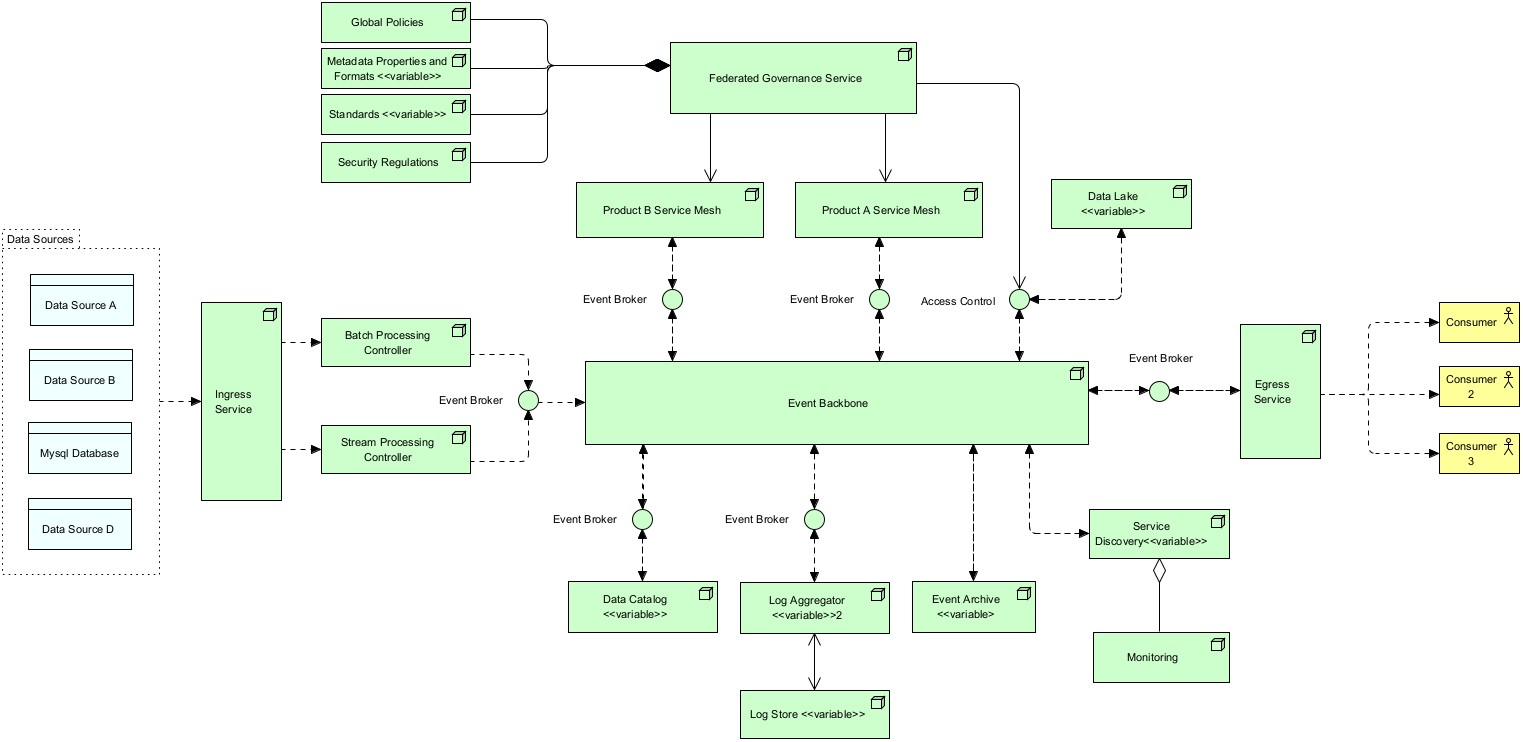
\includegraphics[width=12cm]{Media/Cybermycelium.jpg}
    \label{fig:Cybermycelium}
    \caption{Cybermycelium Big Data Reference Architecture}
\end{figure}

For the purposes of effective modeling and abstraction, we've sub-diagrammed the product domain, which is portrayed in figure \ref{fig:Cybermycelium Product Domain Design}

\begin{figure}[h!]
    \centering
    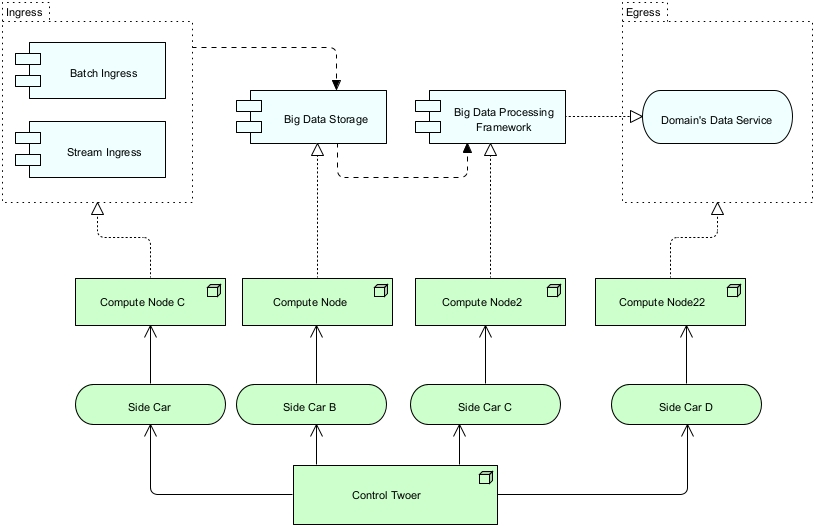
\includegraphics[width=12cm]{Media/Product Domain.jpg}
    \label{fig:Cybermycelium Product Domain Design}
    \caption{Cybermycelium Product Domain Design}
\end{figure}

The main elements are; 

\begin{enumerate}
    \item \textbf{Ingress Service:} The ingress service is responsible for exposing the necessary port and endpoint for the data to flow to the system. Depending on the nature of the request, the ingress service will load balance to either batch processing controller or stream processing controller. It is essential for the ingress service to operate asynchronously to avoid any potential choke points. In addition, ingress handles the SSL termination, and potentially name-based virtual hosting. Ingress has several benefits. Firstly, it helps with security by consolidating by preventing port proliferation and direct access to services. Secondly, it help with performance by distributing requests based on their nature, and SSL termination. 
    \item \textbf{Batch Processing Controller:} Batch processing controller is responsible for dispatching batch events to the event backbone. This service should be a small service (could be a Lambda) with the main responsibility of receiving a request for batch processing and dispatching an event to the event broker. Because the nature of the request is of type batch and has been clearly distinguished by the ingress, batch processing controller can dispatch events in bulk and asynchronously. This is the main difference of this service to stream processing controller. Batch processing controller can execute other non compute-intensive tasks such as scrubbing properties from the given data or adding headers.
    \item \textbf{Stream Processing Controller:} Stream processing controller is responsible for dispatching streaming events to the event backbone through the event broker. This service has been segregated from the batch service as it has to account for a different nature of events. Streams are synchronous in nature, and can require high-throughput. This service is a small service as well, but non-heavy computations such as enabling stream provenance, and one-pass algorithms can be utilized. 
    \item \textbf{Event Broker:} Event brokers are designed to achieve 'inversion of control'. As the company evolves and requirements emerge, the number of nodes in the service increases, new regions of operations may be added, and new events might need to be dispatched. As each service has to communicate with the rest through the event backbone, each service will be required to implement it's own event handling module. This can easily turn into a spaghetti of various implementation by various teams, and can even cause bugs and unexpected behaviors. To overcome this challenge, an event broker is introduced to each main service of the architecture, plus the ingress and egress. Each service connects to its local event broker and publishes and subscribes to events through that broker. One of the key success criteria of the event broker is a unified interface that sits at a right level of abstraction to account for all services of the architecture. Event brokers, being environmentally agnostic can be deployed to any on-premise, private or public infrastructure. Event brokers can also account for more dynamism by learning which events should be routed to which consumer applications.
    \item \textbf{Event Backbone:} This is the heart of the Cybermycelium, facilitating communication among all the nodes. Event backbone in itself should be distributed and ideally clustered to account for the ever-increasing scale of the system. Communication occurs as choreographed events from services analogous to a dance troupe. In a dance troupe, the members respond to the rhythm of the music by moving according to their specific roles. In here, each service (dancer) listens and reacts to the event backbone (music) and takes the required action. This means services are only responsbile for dispatching events in a 'dispatch and forget' model, and subscribe to the topics that are necessary to achieve their ends.
    \item \textbf{Egress Service:}
    \item \textbf{Product Domain:}
    \item \textbf{Federated Governance Service:}
    \item \textbf{Global Policies:}
    \item \textbf{Security Regulations:}
\end{enumerate}

\bibliography{mybibfile}

\end{document}